\documentclass[12pt,a4paper]{article}

% ================= PACOTES =================
\usepackage[utf8]{inputenc}
\usepackage[T1]{fontenc}
\usepackage{lmodern}
% Idioma: usa babel-portugues quando disponivel. Caso o pacote
% texlive-lang-portuguese nao esteja instalado, recorre a rotulos manuais para
% que o documento continue compilando sem erro. Para habilitar a hifenizacao
% correta do portugues: sudo apt install texlive-lang-portuguese
\IfFileExists{brazil.ldf}{%
    \usepackage[brazilian]{babel}%
}{%
    \usepackage[english]{babel}%
    \addto\captionsenglish{%
        \renewcommand{\contentsname}{Sumário}%
        \renewcommand{\figurename}{Figura}%
        \renewcommand{\tablename}{Tabela}%
        \renewcommand{\refname}{Referências}%
        \renewcommand{\abstractname}{Resumo}%
    }%
}
\usepackage{amsmath,amssymb,amsfonts,amsthm}
\usepackage{graphicx}
\usepackage{booktabs}
\usepackage{geometry}
\usepackage{tikz}
\usepackage{cite}
\usepackage{hyperref}
\usepackage{setspace}
\usepackage{indentfirst}

\usetikzlibrary{arrows.meta,positioning,shapes.geometric}

\geometry{a4paper,margin=2.5cm}
\onehalfspacing

\theoremstyle{plain}
\newtheorem{proposicao}{Proposição}
\newtheorem{corolario}[proposicao]{Corolário}
\AtBeginDocument{\renewcommand{\proofname}{Demonstração}}

\hypersetup{
    colorlinks=true,
    linkcolor=black,
    citecolor=black,
    urlcolor=blue,
    pdftitle={Roteamento de Veiculos Multiobjetivo Aplicado ao Ride-Pooling},
    pdfauthor={Bruno Prado Santos, Eduardo Almeida Queiroz, Lucas Cerqueira Portela}
}
\begin{document}

% ============================================================
% CAPA
% ============================================================
\begin{titlepage}
    \begin{center}
        \Large
        \textbf{CENTRO FEDERAL DE EDUCAÇÃO TECNOLÓGICA DE MINAS GERAIS} \\
        \textbf{CÂMPUS V — DIVINÓPOLIS}
        
        \vspace{2cm}
        
        \rule{\linewidth}{0.5mm} \\[0.4cm]
        {\Huge \bfseries Ride-Pooling vs. Transporte Individual: Uma Formulação Multiobjetivo entre Emissões de $\text{CO}_2$ e Qualidade de Serviço ao Usuário} \\[0.1cm]
        \rule{\linewidth}{0.5mm} \\[2cm]

         \begin{figure}[h] 
    \centering
    
\includegraphics[width=0.3\textwidth]{Logo_CEFET-MG.png}
    \label{fig:cefet}
        \end{figure}

        \large
        \textbf{Disciplina:} Otimização Multiobjetivo \\
        \textbf{Professor:} Eduardo Miranda
        
        \vfill

        
        \textbf{Alunos:} \\
        Bruno Prado Santos, Eduardo Almeida Queiroz e Lucas Cerqueira Portela
        
        \vfill
        Divinópolis — MG \\
        \today
    \end{center}
\end{titlepage}

% ============================================================
% RESUMO
% ============================================================
\section*{Resumo}
\addcontentsline{toc}{section}{Resumo}

O crescimento acelerado da frota de veículos individuais em centros urbanos tem intensificado problemas de congestionamento, tempo de deslocamento e emissões de gases de efeito estufa, com destaque para o dióxido de carbono ($\text{CO}_2$). Neste contexto, este trabalho propõe uma metodologia de pesquisa fundamentada no Roteamento de Veículos Multiobjetivo (\textit{Multi-Objective Vehicle Routing Problem} -- MO-VRP), especificamente na variante \textit{Dial-a-Ride Problem} (DARP), para investigar o potencial do \textit{ride-pooling} (transporte compartilhado sob demanda) como alternativa sustentável ao transporte individual motorizado do tipo aplicativo/táxi. O modelo proposto considera dois objetivos ao mesmo tempo e em conflito: minimizar as emissões de $\text{CO}_2$ da frota e minimizar o tempo perdido pelo usuário (desvio de rota e espera no embarque), medido em passageiro-minuto. Mostra-se que os dois objetivos são conflitantes: se ninguém espera e ninguém desvia do caminho direto, os passageiros não podem compartilhar o veículo, e a vantagem do transporte compartilhado desaparece. Esse conflito também aparece nos dados públicos de Cordeau e Laporte: na instância \texttt{pr01}, a solução que só minimiza a distância deixa os passageiros, em média, 45,6 minutos no veículo para viagens que levariam 6,3 minutos no caminho direto --- cerca de 7,2 vezes mais tempo, ou 943 passageiro-minutos de desvio que o modelo clássico de um único objetivo não contabiliza. O documento apresenta a fundamentação teórica, a formulação matemática, a análise das instâncias de teste disponíveis, a estrutura da base de dados e o plano de execução computacional, com validação contra soluções já publicadas e resolução por métodos exatos e metaheurísticas. Trata-se da proposta teórico-metodológica do projeto; os resultados numéricos serão obtidos em etapa posterior.

\textbf{Palavras-chave:} Roteamento de Veículos; Otimização Multiobjetivo; Dial-a-Ride Problem; Ride-Pooling; Qualidade de Serviço; Emissões de $\text{CO}_2$.

\vspace{1cm}

\newpage
\tableofcontents
\newpage

% ============================================================
% SEÇÃO 1 - INTRODUÇÃO
% ============================================================
\section{Introdução e Justificativa}

\subsection{Contextualização}

A mobilidade urbana enfrenta, nas últimas décadas, um desafio estrutural decorrente do crescimento contínuo da frota de veículos motorizados individuais. O aumento do número de deslocamentos realizados por carros de aplicativo e táxis, especialmente em grandes centros urbanos, tem contribuído para o agravamento do congestionamento viário, o aumento do tempo médio de viagem e, de forma particularmente relevante, para o crescimento das emissões de gases de efeito estufa, sobretudo o dióxido de carbono ($\text{CO}_2$). O setor de transportes figura entre os principais responsáveis pelas emissões antrópicas de $\text{CO}_2$, e a operação predominantemente individualizada de veículos -- com baixa taxa de ocupação -- é um dos fatores centrais dessa ineficiência ambiental.

Nesse cenário, soluções de mobilidade compartilhada sob demanda (\textit{ride-pooling}), nas quais múltiplos passageiros com origens e destinos próximos compartilham o mesmo veículo em uma mesma viagem, surgem como alternativa promissora para reduzir tanto a quantidade de veículos em circulação quanto a emissão de poluentes por passageiro transportado. A viabilidade operacional dessas soluções depende, no entanto, de um problema de otimização combinatória não trivial: como determinar as rotas dos veículos compartilhados de forma a atender simultaneamente múltiplas solicitações de passageiros, respeitando restrições de capacidade, janelas de tempo e tempo máximo de viagem tolerável, sem comprometer excessivamente a qualidade do serviço em relação ao atendimento individual?

\subsection{Definição da Problemática}

O problema central investigado neste trabalho pode ser formulado da seguinte maneira: dado um mesmo conjunto de solicitações de viagem (par origem-destino, horário desejado e número de passageiros), como comparar, sob uma perspectiva multiobjetivo, o atendimento por uma frota de veículos privados individuais (capacidade de 1 a 4 passageiros) frente ao atendimento por uma frota de veículos compartilhados sob demanda (capacidade de 8 a 15 passageiros, com agrupamento de múltiplas solicitações em uma mesma rota)?

Essa comparação não pode ser reduzida a um único critério de desempenho. A frota compartilhada tende a reduzir a distância total percorrida e, consequentemente, as emissões de $\text{CO}_2$ do sistema; em contrapartida, ela aumenta necessariamente o tempo de viagem individual de cada passageiro, em razão dos desvios de rota exigidos para atender múltiplas solicitações na mesma viagem. Trata-se, portanto, de um problema genuinamente multiobjetivo, no qual a redução do impacto ambiental está em conflito direto com a qualidade do serviço percebida pelo usuário.

É importante destacar que a literatura clássica de DARP trata o tempo de viagem do passageiro como \textit{restrição} -- um limite superior de tolerância (\textit{maximum ride time}) --, e não como objetivo. Essa escolha de modelagem tem uma consequência que costuma passar desapercebida: a otimização passa a ser indiferente a qualquer degradação de serviço que respeite o limite imposto, ainda que essa degradação seja severa. Como será demonstrado na Seção~\ref{sec:conflito} e quantificado na Seção~\ref{sec:instancias}, as soluções de referência da literatura para as instâncias de \textit{benchmark} do DARP exibem tempos de viagem que chegam a mais de sete vezes o percurso direto do passageiro, justamente porque nada na função objetivo penaliza esse desvio. O presente trabalho promove explicitamente essa dimensão a função objetivo, tornando o \textit{trade-off} entre sustentabilidade e qualidade de serviço um resultado quantitativo do modelo -- expresso por uma Fronteira de Pareto -- em vez de uma premissa implícita na escolha de um parâmetro.

\subsection{Objetivos}

\subsubsection{Objetivo Geral}

Propor e formalizar um modelo de Roteamento de Veículos Multiobjetivo (MO-VRP/\allowbreak MO-DARP) capaz de quantificar o \textit{trade-off} entre emissões de $\text{CO}_2$ e qualidade de serviço ao usuário no atendimento de um mesmo conjunto de demandas de passageiros, comparando uma frota de transporte privado individual a uma frota de transporte compartilhado sob demanda (\textit{ride-pooling}), como subsídio metodológico para avaliação de políticas de mobilidade urbana sustentável.

\subsubsection{Objetivos Específicos}

\begin{itemize}
    \item Revisar a literatura científica sobre Roteamento de Veículos com múltiplos objetivos, com ênfase nas variantes \textit{Dial-a-Ride Problem} (DARP), \textit{Green Vehicle Routing Problem} (G-VRP) e no tratamento de critérios de qualidade de serviço;
    \item Formalizar matematicamente o modelo de MO-DARP com dois objetivos, incluindo variáveis de decisão, funções objetivo (emissão de $\text{CO}_2$ e tempo perdido pelo usuário) e restrições, e demonstrar a relação de conflito entre os objetivos;
    \item Analisar estruturalmente as instâncias de \textit{benchmark} disponíveis para o DARP, verificando sua adequação ao modelo proposto e identificando os parâmetros que necessitam de calibração ou arbitragem;
    \item Definir a estrutura lógica da base de dados necessária para a instanciação do modelo, contemplando nós de coleta e entrega, coordenadas, demandas, janelas de tempo, instantes desejados de embarque e matrizes de distância/tempo;
    \item Estabelecer o plano de execução computacional do projeto, incluindo o procedimento de validação do avaliador de soluções, as estratégias de resolução (métodos exatos e metaheurísticas) e as métricas de avaliação das fronteiras obtidas.
\end{itemize}

% ============================================================
% SEÇÃO 2 - FUNDAMENTAÇÃO TEÓRICA
% ============================================================
\section{Fundamentação Teórica e Trabalhos Relacionados}

\subsection{O Problema de Roteamento de Veículos (VRP) e suas Variantes}

O Problema de Roteamento de Veículos (\textit{Vehicle Routing Problem} -- VRP) consiste, em sua forma clássica, em determinar um conjunto de rotas de custo mínimo para uma frota de veículos baseada em um depósito único, de modo a atender a demanda de um conjunto de clientes, respeitando restrições de capacidade veicular. Trata-se de um problema NP-difícil, generalização do Problema do Caixeiro Viajante (TSP) para múltiplos veículos, amplamente estudado desde os trabalhos seminais de Dantzig e Ramser.

Diversas variantes do VRP foram desenvolvidas para incorporar características operacionais específicas de aplicações reais, das quais três são particularmente relevantes para este trabalho:

\begin{itemize}
    \item \textbf{VRP com Janelas de Tempo (VRPTW):} incorpora a restrição de que cada cliente deve ser atendido dentro de um intervalo de tempo pré-definido $[e_i, l_i]$, refletindo situações em que o atendimento fora desse intervalo é inviável ou penalizado;
    \item \textbf{\textit{Dial-a-Ride Problem} (DARP):} generaliza o VRP com Coleta e Entrega (\textit{Pickup and Delivery Problem}) para o transporte de pessoas, introduzindo, além das janelas de tempo, restrições de emparelhamento (o mesmo veículo deve atender coleta e entrega da mesma solicitação), precedência (a coleta deve ocorrer antes da entrega) e tempo máximo de viagem por passageiro (\textit{ride time}), de modo a garantir um nível mínimo de qualidade de serviço ao usuário transportado~\cite{cordeau2003,cordeau2006};
    \item \textbf{VRP Verde (\textit{Green VRP} -- G-VRP):} incorpora explicitamente objetivos e/ou restrições ambientais ao modelo clássico de roteamento, tipicamente por meio da minimização do consumo de combustível ou das emissões de poluentes, muitas vezes modeladas como função da distância percorrida, da carga transportada e da velocidade do veículo~\cite{lin2014}.
\end{itemize}

O modelo proposto neste trabalho integra essas três variantes: a estrutura de coleta-entrega e restrições de qualidade de serviço do DARP, as janelas de tempo do VRPTW e a dimensão ambiental do G-VRP, tratada sob a ótica da otimização multiobjetivo.

\subsection{Critérios de Qualidade de Serviço em DARP}

A tensão entre eficiência operacional e qualidade de serviço é reconhecida na literatura de DARP como sua característica definidora. Molenbruch, Braekers e Caris~\cite{molenbruch2017}, em revisão sistemática e proposta de tipologia para o problema, identificam que a grande maioria dos trabalhos trata os critérios de nível de serviço como restrições (janelas de tempo, tempo máximo a bordo, espera máxima), enquanto apenas uma fração minoritária os incorpora diretamente na função objetivo. Os autores apontam explicitamente a abordagem multiobjetivo como uma das direções mais promissoras e menos exploradas do campo.

Parragh et al.~\cite{parragh2009} propuseram uma das primeiras abordagens explicitamente biobjetivo para o DARP, minimizando simultaneamente a distância total percorrida e a inconveniência média do usuário, esta última definida como combinação do tempo de espera e do tempo excedente a bordo. O trabalho emprega um método em duas fases, combinando $\varepsilon$-restrito com uma heurística de busca em vizinhança variável, e demonstra que as duas medidas produzem fronteiras de Pareto amplas -- evidência direta de que os critérios são efetivamente conflitantes.

Paquette et al.~\cite{paquette2013} aprofundaram essa discussão ao articular análise multicritério e busca tabu para o DARP, argumentando que a redução da qualidade de serviço a um único limite paramétrico de tolerância descarta informação relevante para o decisor. Os autores defendem que a qualidade de serviço em transporte de pessoas é intrinsecamente multidimensional e que sua explicitação como objetivo, e não como restrição, é condição para que o \textit{trade-off} seja avaliado de forma consciente. O presente trabalho adota essa posição metodológica, particularizando-a para o contexto de comparação entre frotas e substituindo o critério de distância pelo de emissão de $\text{CO}_2$.

\subsection{Trabalhos Relacionados em Roteamento Ambiental e Multiobjetivo}

Bektaş e Laporte~\cite{bektas2011} introduziram o \textit{Pollution-Routing Problem} (PRP), extensão do VRP clássico cuja função objetivo passa a incorporar, além da distância percorrida, o consumo de combustível, as emissões de gases de efeito estufa e os custos associados ao tempo de viagem. O PRP é considerado o trabalho fundador da linha de pesquisa que relaciona explicitamente decisões de roteamento e velocidade ao impacto ambiental do transporte rodoviário, e fornece a base conceitual para o cálculo de emissões utilizado neste projeto.

Demir, Bektaş e Laporte~\cite{demir2014} propuseram a versão com dois objetivos do PRP, na qual minimizar o consumo de combustível e minimizar o tempo total de condução são tratados como critérios conflitantes, resolvidos por uma heurística de busca em vizinhança ampla adaptativa (ALNS), combinada a métodos de geração da fronteira de Pareto aplicados depois da busca (soma ponderada, $\varepsilon$-restrito e método híbrido). Esse trabalho é particularmente relevante por um aviso metodológico: se dois objetivos crescem juntos com a mesma quantidade física -- por exemplo distância, consumo e custo por quilômetro -- eles não são realmente conflitantes, e a otimização simultânea acaba em um único ponto, e não em uma curva de equilíbrio. Para haver conflito de verdade, é preciso um mecanismo de oposição: no PRP esse papel é da velocidade; neste trabalho, é o fato de que agrupar passageiros na mesma viagem reduz emissão, mas aumenta o tempo de cada um.

Petrovic, Islam e Trautrims~\cite{petrovic2023} abordaram o Problema de Roteamento com Coleta e Entrega Simultâneas (VRPSPD) sob a perspectiva multiobjetivo, considerando a minimização da distância percorrida e do consumo de combustível como dois objetivos distintos, evitando a combinação prévia em uma única função ponderada. O modelo foi resolvido por meio do algoritmo NSGA-II, com uma heurística construtiva baseada no método de decisão multicritério TOPSIS para geração da população inicial.

Jozefowiez, Semet e Talbi~\cite{jozefowiez2008} apresentaram a revisão de referência sobre problemas de roteamento multiobjetivo, sistematizando as motivações para a extensão do VRP mono-objetivo e classificando os critérios adicionais usualmente empregados, entre eles balanceamento de carga, nível de serviço e impacto ambiental. Lin et al.~\cite{lin2014}, por sua vez, revisaram especificamente a literatura de \textit{Green Vehicle Routing Problem}, propondo uma classificação do campo em três subcategorias e discutindo a evolução do objetivo tradicional de minimização de custos para a incorporação simultânea de critérios econômicos e ambientais.

Por fim, Assis et al.~\cite{assis2013} trataram o problema de roteamento de veículos multiobjetivo com coleta seletiva, no qual a restrição de atendimento integral das demandas de coleta é convertida em função objetivo. Além de ilustrar um mecanismo geral de construção de problemas multiobjetivo com conflito garantido -- a conversão de restrição em objetivo --, o trabalho é adotado neste projeto como referência metodológica para o protocolo experimental, em particular quanto ao conjunto de métricas de avaliação de fronteiras (hipervolume, cobertura e cardinalidade), à geração dos pontos extremos da fronteira a partir de soluções mono-objetivo e ao delineamento estatístico em blocos aleatorizados para comparação de algoritmos.

% ============================================================
% SEÇÃO 3 - METODOLOGIA
% ============================================================
\section{Metodologia e Modelagem Proposta}

\subsection{Descrição do Cenário}
\label{sec:cenario}

O cenário de estudo consiste em um conjunto fixo de solicitações de viagem de passageiros, cada uma definida por um ponto de coleta (origem), um ponto de entrega (destino), um número de passageiros e um instante desejado de embarque. Esse mesmo conjunto de solicitações é submetido a duas configurações alternativas de frota, avaliadas de forma comparativa e resolvidas de forma independente:

\begin{itemize}
    \item \textbf{Cenário I -- Frota Privada Individual:} veículos de baixa capacidade ($Q = 4$), representativos de carros de aplicativo/táxi, com fator de emissão reduzido por quilômetro rodado;
    \item \textbf{Cenário C -- Frota Compartilhada sob Demanda:} veículos de capacidade intermediária ($Q$ entre 8 e 15), do tipo van ou micro-ônibus, com fator de emissão por quilômetro superior, mas capazes de atender múltiplas solicitações simultaneamente por meio do agrupamento de rotas (\textit{ride-pooling}).
\end{itemize}

Cada cenário é resolvido separadamente sobre o mesmo conjunto de viagens, produzindo uma Fronteira de Pareto própria. A comparação entre as duas fronteiras é o resultado central da pesquisa: ela mostra quantos gramas de $\text{CO}_2$ o compartilhamento economiza em relação ao atendimento individual e, sobretudo, quanto tempo extra o usuário precisa aceitar para cada grama economizado.

Adota-se, dentro de cada cenário, uma frota de um único tipo de veículo. Assim, as diferenças ao longo de cada fronteira vêm das rotas e do agrupamento de passageiros, e não da mistura de tipos de veículo.

\subsection{Formulação Matemática}

\subsubsection{Conjuntos e Índices}

Seja $n$ o número de solicitações de passageiros. Define-se:
\begin{itemize}
    \item $P = \{1, \dots, n\}$: conjunto dos nós de coleta (\textit{pickup});
    \item $D = \{n+1, \dots, 2n\}$: conjunto dos nós de entrega (\textit{delivery}), onde o nó $n+i$ corresponde ao ponto de entrega da solicitação cujo ponto de coleta é o nó $i$;
    \item $N = P \cup D$: conjunto dos nós de atendimento;
    \item $\{0,\ 2n+1\}$: nós que representam, respectivamente, a saída e o retorno ao depósito (coincidentes fisicamente no mesmo ponto geográfico);
    \item $V = N \cup \{0,\ 2n+1\}$: conjunto de todos os nós do problema;
    \item $A = \{(i,j) : i,j \in V,\ i \neq j\}$: conjunto de arcos possíveis entre os nós;
    \item $K$: conjunto de veículos disponíveis, homogêneos dentro de cada cenário, com $m = |K|$.
\end{itemize}

\subsubsection{Parâmetros}

\begin{itemize}
    \item $d_{ij}$: distância entre os nós $i$ e $j$;
    \item $t_{ij}$: tempo de deslocamento entre os nós $i$ e $j$;
    \item $\phi$: fator de emissão de $\text{CO}_2$ por unidade de distância (g $\text{CO}_2$/km), específico do cenário de frota;
    \item $q_i$: número de passageiros da solicitação associada ao nó $i$, com $q_{n+i} = -q_i$ para $i \in P$ e $q_0 = q_{2n+1} = 0$;
    \item $Q$: capacidade máxima do veículo, específica do cenário de frota;
    \item $[e_i,\ l_i]$: janela de tempo aceitável para atendimento do nó $i$;
    \item $s_i$: tempo de serviço (embarque/desembarque) no nó $i$, com $s_i > 0$ para $i \in N$;
    \item $\rho_i$: instante desejado de embarque da solicitação $i \in P$, com $\rho_i = e_i$;
    \item $\bar{t}_i = t_{i,(n+i)}$: tempo de percurso direto da solicitação $i \in P$, parâmetro derivado;
    \item $L_i = \alpha\,\bar{t}_i$: tempo máximo tolerável a bordo para a solicitação $i \in P$, proporcional ao percurso direto, com $\alpha > 1$;
    \item $T_{max}$: duração máxima de rota permitida para cada veículo;
    \item $M_{ij}$: constante suficientemente grande, definida como $M_{ij} = \max\{0,\ l_i + s_i + t_{ij} - e_j\}$.
\end{itemize}

Duas observações sobre a parametrização. Primeiro, o fator de emissão é denotado por $\phi$, e não pela letra $\varepsilon$ usual na literatura de G-VRP, a fim de evitar colisão de notação com o método $\varepsilon$-restrito empregado na Seção~\ref{sec:resolucao}. Segundo, o tempo máximo a bordo $L_i$ é definido \textit{proporcionalmente} ao percurso direto de cada solicitação, e não como uma constante global. Essa escolha é justificada na Seção~\ref{sec:parametros}: um limite global uniforme impõe tolerâncias radicalmente distintas a viagens curtas e longas e, nas instâncias de \textit{benchmark} existentes, corresponde a fatores de inflação sem correspondência com o comportamento real de usuários de transporte sob demanda.

\subsubsection{Variáveis de Decisão}

\begin{align}
x_{ijk} &\in \{0,1\}: \text{igual a 1 se o veículo } k \text{ percorre o arco } (i,j),\ 0 \text{ caso contrário} \\
y_{k}   &\in \{0,1\}: \text{igual a 1 se o veículo } k \text{ é utilizado},\ 0 \text{ caso contrário} \\
B_{i}   &\geq 0: \text{instante de início do atendimento no nó } i \in N \\
B^{\text{ini}}_{k},\ B^{\text{fim}}_{k} &\geq 0: \text{instantes de saída e de retorno ao depósito do veículo } k \\
w_{i}   &\geq 0: \text{número de passageiros a bordo imediatamente após a visita ao nó } i \in N \\
R_{i}   &\geq 0: \text{tempo a bordo (\textit{ride time}) do passageiro da solicitação } i \in P
\end{align}

As variáveis $B_i$, $w_i$ e $R_i$ possuem índice único, sem referência ao veículo. Isso é possível porque cada nó de atendimento é visitado exatamente uma vez, por exatamente um veículo, e evita a inconsistência de exigir o cumprimento de janelas de tempo para veículos que não visitam o nó em questão. Os instantes de saída e retorno ao depósito, por serem específicos de cada rota, permanecem indexados em $k$.

\subsubsection{Funções Objetivo}

\textbf{Objetivo ambiental --- minimização das emissões totais de $\text{CO}_2$:}
\begin{equation}
\min\ f_1 = \sum_{k \in K} \sum_{(i,j) \in A} \phi\, d_{ij}\, x_{ijk}
\label{eq:f1}
\end{equation}

\textbf{Objetivo de serviço --- minimização do tempo perdido pelo usuário:}
\begin{equation}
\min\ f_2 = \sum_{i \in P} q_i \Big[ \underbrace{(R_i - \bar{t}_i)}_{\text{desvio de rota}} \;+\; \underbrace{(B_i - \rho_i)}_{\text{espera no embarque}} \Big]
\label{eq:f2}
\end{equation}

A função $f_2$ é expressa em passageiro-minuto e agrega as duas parcelas de tempo que o usuário perde em relação ao serviço ideal: o excedente a bordo, decorrente dos desvios necessários para atender outras solicitações, e a espera entre o instante desejado de embarque e o embarque efetivo. Três decisões de modelagem merecem registro.

A primeira é o uso do tempo \textit{excedente} $(R_i - \bar{t}_i)$, e não do tempo absoluto a bordo $R_i$. O percurso direto $\bar{t}_i$ é uma constante irredutível, independente de qualquer decisão de roteamento; mantê-la na função objetivo apenas adiciona um deslocamento constante que comprime a variação relativa do objetivo e dificulta a interpretação da fronteira.

A segunda é a ponderação por $q_i$. A unidade resultante, passageiro-minuto, mede o tempo perdido no conjunto dos usuários e evita que uma viagem de quatro pessoas pese o mesmo que uma de uma só pessoa.

A terceira é a ausência de um peso relativo entre as duas parcelas. Ambas são medidas em minutos e representam tempo perdido pelo usuário, o que dispensa a arbitragem de um coeficiente de conversão. Registre-se que a inclusão da parcela de espera não é redundante com a de desvio: sem ela, o modelo admitiria soluções nas quais um único veículo atende todas as solicitações em sequência, com desvio nulo e distância baixa, ao custo de esperas arbitrariamente longas.

\paragraph{Tratamento do custo operacional.} O custo operacional não entra como objetivo. Com veículos do mesmo tipo, esse custo acompanha a distância total --- a mesma quantidade que já define $f_1$ --- e, se fosse um terceiro objetivo, repetiria o primeiro, em vez de revelar um equilíbrio novo, ponto contra o qual Demir et al.~\cite{demir2014} advertem. O custo é, portanto, calculado depois, para cada solução da fronteira, como indicador econômico:
\begin{equation}
C = \sum_{k \in K}\Big[ F\, y_k + c \sum_{(i,j) \in A} d_{ij}\, x_{ijk} + c^{h}\big(B^{\text{fim}}_k - B^{\text{ini}}_k\big)\Big]
\label{eq:custo}
\end{equation}
onde $F$ é o custo fixo por veículo utilizado, $c$ o custo por unidade de distância e $c^{h}$ o custo por unidade de tempo de operação (remuneração do condutor).

\subsubsection{Restrições}

\textbf{Atendimento único de cada solicitação:}
\begin{equation}
\sum_{k \in K} \sum_{j \in V} x_{ijk} = 1, \qquad \forall i \in P
\end{equation}

\textbf{Emparelhamento coleta-entrega (mesmo veículo atende ambos os nós da solicitação):}
\begin{equation}
\sum_{j \in V} x_{ijk} - \sum_{j \in V} x_{(n+i)jk} = 0, \qquad \forall i \in P,\ \forall k \in K
\end{equation}

\textbf{Conservação de fluxo em cada nó de atendimento:}
\begin{equation}
\sum_{i \in V,\, i \neq h} x_{ihk} - \sum_{j \in V,\, j \neq h} x_{hjk} = 0, \qquad \forall h \in N,\ \forall k \in K
\end{equation}

\textbf{Saída e retorno ao depósito, condicionados à utilização do veículo:}
\begin{equation}
\sum_{j \in P} x_{0jk} = y_k, \qquad \forall k \in K
\label{eq:saida}
\end{equation}
\begin{equation}
\sum_{i \in D} x_{i,(2n+1),k} = y_k, \qquad \forall k \in K
\end{equation}

\textbf{Consistência temporal ao longo da rota:}
\begin{equation}
B_j \geq B_i + s_i + t_{ij} - M_{ij}\Big(1 - \sum_{k \in K} x_{ijk}\Big), \qquad \forall (i,j) \in A,\ i,j \in N
\end{equation}
\begin{equation}
B_j \geq B^{\text{ini}}_k + t_{0j} - M_{0j}\,(1 - x_{0jk}), \qquad \forall j \in P,\ \forall k \in K
\end{equation}
\begin{equation}
B^{\text{fim}}_k \geq B_i + s_i + t_{i,(2n+1)} - M_{i,(2n+1)}\,(1 - x_{i,(2n+1),k}), \qquad \forall i \in D,\ \forall k \in K
\end{equation}

\textbf{Janelas de tempo:}
\begin{equation}
e_i \leq B_i \leq l_i, \qquad \forall i \in N
\label{eq:janelas}
\end{equation}

\textbf{Precedência e tempo a bordo:}
\begin{equation}
R_i = B_{(n+i)} - \big(B_i + s_i\big), \qquad \forall i \in P
\end{equation}
\begin{equation}
\bar{t}_i \leq R_i \leq L_i, \qquad \forall i \in P
\label{eq:ridetime}
\end{equation}

\textbf{Capacidade do veículo:}
\begin{equation}
w_j \geq w_i + q_j - Q\Big(1 - \sum_{k \in K} x_{ijk}\Big), \qquad \forall (i,j) \in A,\ i,j \in N
\end{equation}
\begin{equation}
w_j \leq q_j + Q\Big(1 - \sum_{k \in K} x_{0jk}\Big), \qquad \forall j \in P
\end{equation}
\begin{equation}
\max\{0,\ q_i\} \leq w_i \leq \min\{Q,\ Q + q_i\}, \qquad \forall i \in N
\end{equation}

\textbf{Duração máxima da rota:}
\begin{equation}
B^{\text{fim}}_k - B^{\text{ini}}_k \leq T_{max}, \qquad \forall k \in K
\end{equation}

\textbf{Natureza das variáveis:}
\begin{equation}
x_{ijk} \in \{0,1\}, \quad y_k \in \{0,1\}, \quad B_i,\ w_i,\ R_i \geq 0
\end{equation}

Observe-se que a restrição~\eqref{eq:ridetime} garante a precedência entre coleta e entrega de forma implícita: como $\bar{t}_i > 0$ e $R_i \geq \bar{t}_i$, tem-se necessariamente $B_{(n+i)} > B_i$. A restrição~\eqref{eq:saida} emprega igualdade a $y_k$, e não a 1, de modo que veículos não utilizados permaneçam inativos sem tornar o modelo infactível; e a restrição~\eqref{eq:janelas} é imposta sobre variáveis de índice único, evitando a exigência --- infactível quando $e_i > 0$ --- de que todos os veículos cumpram a janela de todos os nós.

\subsection{Conflito entre as Funções Objetivo}
\label{sec:conflito}

A condição para que o problema seja genuinamente multiobjetivo é que os critérios se oponham estruturalmente, e não apenas por efeito de parametrização. Esta seção estabelece essa oposição em duas etapas: uma proposição que caracteriza o extremo de serviço perfeito e uma verificação empírica do extremo ambiental.

\begin{proposicao}[Serviço perfeito proíbe o agrupamento]
\label{prop:conflito}
Seja $S$ uma solução viável do modelo com $f_2(S) = 0$. Então, para toda solicitação $i \in P$, o veículo que a atende não visita nenhum nó entre a coleta $i$ e a entrega $n+i$. Consequentemente, nenhum veículo transporta mais de uma solicitação por vez, e a capacidade $Q > \max_{i \in P} q_i$ é irrelevante em $S$.
\end{proposicao}

\begin{proof}
Como $q_i > 0$ e ambas as parcelas de~\eqref{eq:f2} são não negativas --- a primeira por~\eqref{eq:ridetime} e a segunda porque $\rho_i = e_i \leq B_i$ por~\eqref{eq:janelas} ---, a igualdade $f_2(S) = 0$ implica $R_i = \bar{t}_i$ para toda solicitação $i \in P$.

Suponha, por absurdo, que o veículo que atende a solicitação $i$ visite algum nó $h \in N$, com $h \notin \{i,\ n+i\}$, entre a coleta e a entrega de $i$. O tempo a bordo do passageiro $i$ inclui então o deslocamento até $h$, o tempo de serviço em $h$ e o deslocamento de $h$ até $n+i$, de modo que
\[
R_i \;\geq\; t_{ih} + s_h + t_{h,(n+i)} \;\geq\; t_{i,(n+i)} + s_h \;=\; \bar{t}_i + s_h \;>\; \bar{t}_i,
\]
onde a segunda desigualdade decorre da desigualdade triangular sobre a matriz de tempos e a última de $s_h > 0$. Isso contradiz $R_i = \bar{t}_i$. Logo nenhum nó é visitado entre $i$ e $n+i$.

Como isso vale para toda solicitação, cada rota é uma concatenação de blocos completos do tipo coleta-entrega, e a carga do veículo nunca excede $\max_{i \in P} q_i$.
\end{proof}

\begin{corolario}
Toda a vantagem estrutural da frota compartilhada sobre a frota individual encontra-se estritamente na região $f_2 > 0$ do espaço de objetivos.
\end{corolario}

A Proposição~\ref{prop:conflito} estabelece que o extremo de serviço perfeito anula o agrupamento. Resta verificar a direção oposta: que o agrupamento reduz de fato $f_1$ de forma substancial, e que a redução de $f_1$ implica degradação de $f_2$. Essa segunda direção é de natureza empírica --- depende da geometria da instância --- e é quantificada na Seção~\ref{sec:instancias} a partir de soluções publicadas na literatura, além de ilustrada pelo exemplo mínimo da Seção~\ref{sec:exemplo}. Em conjunto, as duas direções caracterizam $f_1$ e $f_2$ como objetivos conflitantes: não existe solução que otimize ambos simultaneamente, e o conjunto de soluções eficientes forma uma fronteira não trivial.

Vale contrastar esse mecanismo com o do modelo clássico que minimiza ao mesmo tempo emissão e custo. Com veículos do mesmo tipo, emissão e custo por quilômetro crescem juntos com a distância; otimizar os dois ao mesmo tempo leva a um único ponto, e não a uma curva de equilíbrio. O conflito deste trabalho não depende de ajustar parâmetros: ele vem do fato de que o caminho mais curto entre dois pontos não passa por um terceiro, e de que embarcar ou desembarcar alguém leva tempo. Isso vale para qualquer conjunto de viagens.

\subsection{Exemplo Mínimo do \textit{Trade-off}}
\label{sec:exemplo}

Considere um depósito na origem e duas solicitações com $q_1 = q_2 = 1$, coletas em $p_1 = (1,1)$ e $p_2 = (2,-1)$ e entregas em $d_1 = (9,1)$ e $d_2 = (10,-1)$, com tempos de serviço desprezíveis e velocidade unitária. Ambas as solicitações têm percurso direto $\bar{t}_1 = \bar{t}_2 = 8$. A Tabela~\ref{tab:exemplo} apresenta as três estratégias de atendimento e a Figura~\ref{fig:tradeoff} ilustra as duas relevantes.

\begin{table}[htbp]
\centering
\caption{Avaliação de três estratégias para o exemplo mínimo de duas solicitações}
\label{tab:exemplo}
\begin{tabular}{@{}llrrl@{}}
\toprule
\textbf{Estratégia} & \textbf{Rota(s)} & $\boldsymbol{f_1/\phi}$ & $\boldsymbol{f_2}$ & \textbf{Situação} \\
\midrule
Dedicada    & $0\,p_1 d_1\,0$ \ e \ $0\,p_2 d_2\,0$ & 38,76 & 0,00 & dominada \\
Sequencial  & $0\,p_1 d_1 p_2 d_2\,0$               & 34,74 & 0,00 & eficiente \\
Agrupada    & $0\,p_1 p_2 d_1 d_2\,0$               & 23,22 & 3,03 & eficiente \\
\bottomrule
\end{tabular}
\end{table}

A estratégia dedicada é pior que a sequencial, porque a sequencial chega ao mesmo serviço perfeito com menor distância, evitando voltas desnecessárias ao depósito. Restam duas soluções que não superam uma à outra: a sequencial, em que o usuário não perde tempo, e a agrupada, que reduz a distância --- e portanto a emissão --- em 33\%, ao custo de 3,03 passageiro-minutos de desvio. A solução sequencial obedece à Proposição~\ref{prop:conflito}: nenhum veículo carrega dois passageiros ao mesmo tempo, de modo que a capacidade da van não ajuda nesse extremo. Com mais viagens e origens mais próximas, os desvios se acumulam e a fronteira se preenche com graus intermediários de agrupamento.

\begin{figure}[htbp]
\centering
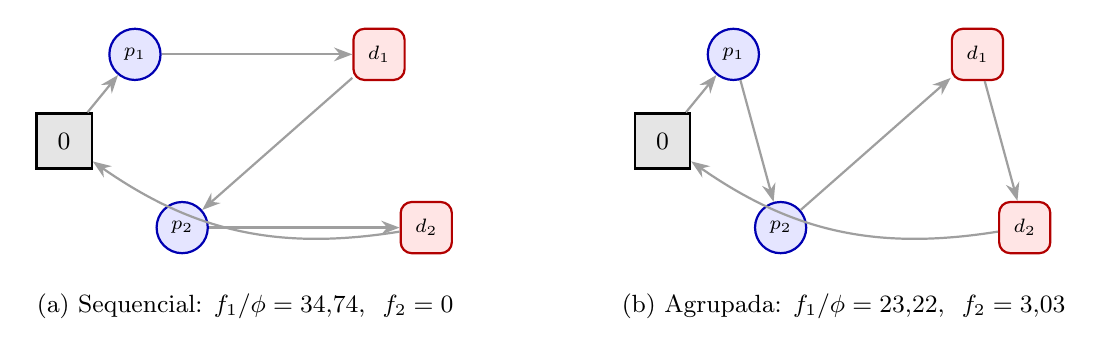
\begin{tikzpicture}[
    >=Stealth,
    deposito/.style={rectangle, draw=black, thick, fill=gray!20, minimum size=0.7cm, font=\small},
    coleta/.style={circle, draw=blue!70!black, thick, fill=blue!10, minimum size=0.65cm, font=\scriptsize},
    entrega/.style={rectangle, rounded corners, draw=red!70!black, thick, fill=red!10, minimum size=0.65cm, font=\scriptsize},
    arco/.style={->, thick, gray!75},
    scale=1.0
]
% ---------- (a) Sequencial ----------
\begin{scope}[xshift=0cm]
\node[deposito] (d0) at (0,0) {$0$};
\node[coleta]   (a1) at (0.9,1.1) {$p_1$};
\node[entrega]  (b1) at (4.0,1.1) {$d_1$};
\node[coleta]   (a2) at (1.5,-1.1) {$p_2$};
\node[entrega]  (b2) at (4.6,-1.1) {$d_2$};
\draw[arco] (d0) -- (a1);
\draw[arco] (a1) -- (b1);
\draw[arco] (b1) -- (a2);
\draw[arco] (a2) -- (b2);
\draw[arco] (b2) to[bend left=22] (d0);
\node[font=\small] at (2.3,-2.1) {(a) Sequencial: $f_1/\phi = 34{,}74$, \ $f_2 = 0$};
\end{scope}
% ---------- (b) Agrupada ----------
\begin{scope}[xshift=7.6cm]
\node[deposito] (e0) at (0,0) {$0$};
\node[coleta]   (c1) at (0.9,1.1) {$p_1$};
\node[entrega]  (f1) at (4.0,1.1) {$d_1$};
\node[coleta]   (c2) at (1.5,-1.1) {$p_2$};
\node[entrega]  (f2) at (4.6,-1.1) {$d_2$};
\draw[arco] (e0) -- (c1);
\draw[arco] (c1) -- (c2);
\draw[arco] (c2) -- (f1);
\draw[arco] (f1) -- (f2);
\draw[arco] (f2) to[bend left=22] (e0);
\node[font=\small] at (2.3,-2.1) {(b) Agrupada: $f_1/\phi = 23{,}22$, \ $f_2 = 3{,}03$};
\end{scope}
\end{tikzpicture}
\caption{Representação esquemática (fora de escala) das duas soluções eficientes do exemplo mínimo. Em (a), cada passageiro é levado diretamente ao destino e não perde tempo extra, mas o veículo percorre o corredor três vezes. Em (b), as duas coletas são feitas antes das entregas, o que reduz a distância em 33\% e introduz desvio para ambos os passageiros. As distâncias exatas constam da Tabela~\ref{tab:exemplo}.}
\label{fig:tradeoff}
\end{figure}

\subsection{Estrutura Visual em Grafo}

O problema pode ser representado formalmente como um grafo direcionado $G = (V, A)$, no qual os nós representam o depósito e os pontos de coleta/entrega de passageiros, e os arcos representam os deslocamentos possíveis entre esses pontos, ponderados por sua distância (ou tempo associado). A Figura~\ref{fig:grafo_darp} ilustra essa estrutura para uma instância reduzida com três solicitações de passageiros ($n=3$).

\begin{figure}[htbp]
\centering
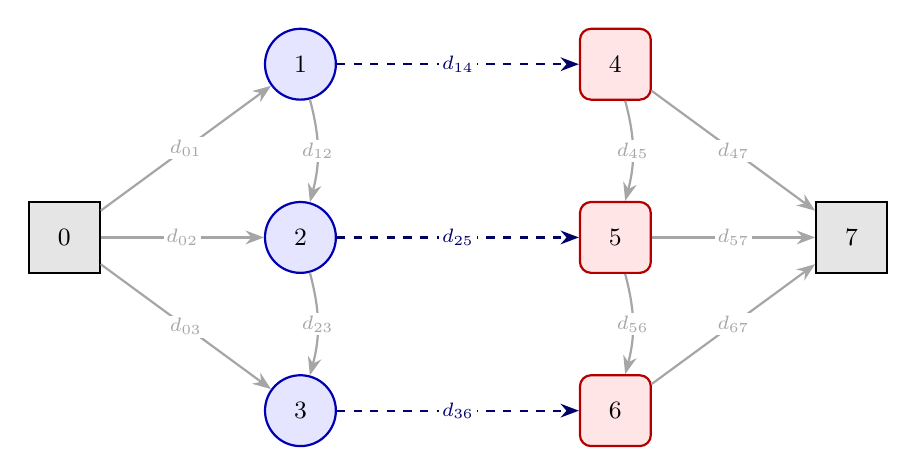
\begin{tikzpicture}[
    >=Stealth,
    node distance=2.3cm,
    deposito/.style={rectangle, draw=black, thick, fill=gray!20, minimum size=0.9cm, font=\small},
    coleta/.style={circle, draw=blue!70!black, thick, fill=blue!10, minimum size=0.9cm, font=\small},
    entrega/.style={rectangle, rounded corners, draw=red!70!black, thick, fill=red!10, minimum size=0.9cm, font=\small},
    arco/.style={->, thick, gray!70},
    rotulo/.style={font=\scriptsize, fill=white, inner sep=1pt}
]

% Depósito
\node[deposito] (dep0) at (0,0) {$0$};

% Nós de coleta
\node[coleta] (p1) at (3,2.2) {$1$};
\node[coleta] (p2) at (3,0) {$2$};
\node[coleta] (p3) at (3,-2.2) {$3$};

% Nós de entrega
\node[entrega] (d1) at (7,2.2) {$4$};
\node[entrega] (d2) at (7,0) {$5$};
\node[entrega] (d3) at (7,-2.2) {$6$};

% Depósito de retorno
\node[deposito] (dep7) at (10,0) {$7$};

% Arcos do depósito para coletas
\draw[arco] (dep0) -- node[rotulo]{$d_{01}$} (p1);
\draw[arco] (dep0) -- node[rotulo]{$d_{02}$} (p2);
\draw[arco] (dep0) -- node[rotulo]{$d_{03}$} (p3);

% Arcos coleta -> entrega (emparelhamento)
\draw[arco, blue!40!black, dashed] (p1) -- node[rotulo]{$d_{14}$} (d1);
\draw[arco, blue!40!black, dashed] (p2) -- node[rotulo]{$d_{25}$} (d2);
\draw[arco, blue!40!black, dashed] (p3) -- node[rotulo]{$d_{36}$} (d3);

% Arcos entre coletas (agrupamento na frota compartilhada)
\draw[arco] (p1) to[bend left=15] node[rotulo]{$d_{12}$} (p2);
\draw[arco] (p2) to[bend left=15] node[rotulo]{$d_{23}$} (p3);

% Arcos entre entregas
\draw[arco] (d1) to[bend left=15] node[rotulo]{$d_{45}$} (d2);
\draw[arco] (d2) to[bend left=15] node[rotulo]{$d_{56}$} (d3);

% Arcos de entrega para depósito de retorno
\draw[arco] (d1) -- node[rotulo]{$d_{47}$} (dep7);
\draw[arco] (d2) -- node[rotulo]{$d_{57}$} (dep7);
\draw[arco] (d3) -- node[rotulo]{$d_{67}$} (dep7);

\end{tikzpicture}
\caption{Representação do problema como grafo direcionado $G=(V,A)$: nós quadrados cinza representam o depósito (saída, nó $0$, e retorno, nó $2n+1=7$), círculos azuis representam os nós de coleta $P=\{1,2,3\}$, e retângulos vermelhos arredondados representam os nós de entrega correspondentes $D=\{4,5,6\}$. Arcos tracejados indicam o par coleta-entrega de uma mesma solicitação. Os arcos entre coletas distintas ($d_{12}$, $d_{23}$) são os que permitem agrupar viagens no mesmo veículo e, por consequência, o equilíbrio estudado neste trabalho.}
\label{fig:grafo_darp}
\end{figure}

\subsection{Análise das Instâncias de Teste}
\label{sec:instancias}

Os arquivos de teste usados na literatura do DARP, disponibilizados por Cordeau e Laporte, foram abertos e conferidos um a um, para saber se servem ao modelo deste trabalho. Eles estão em duas pastas no repositório da HEC Montréal: uma ligada ao artigo de busca tabu~\cite{cordeau2003} e outra ao artigo de \textit{branch-and-cut}~\cite{cordeau2006}.

\subsubsection{Como os arquivos estão organizados}

Cada arquivo começa com uma linha de cinco números e, em seguida, uma linha por ponto do mapa (depósito, coletas e entregas). Os cinco números da primeira linha são, nesta ordem: quantidade de veículos, um segundo número cujo significado muda de pasta para pasta, duração máxima da jornada, capacidade do veículo e tempo máximo que o passageiro pode ficar a bordo.

A diferença entre as pastas é fácil de passar despercebida e, se for ignorada, o programa lê o problema errado:

\begin{itemize}
    \item Na pasta de \textit{branch-and-cut} (famílias \texttt{a} e \texttt{b}), o segundo número é a \textbf{quantidade de viagens}. O depósito aparece duas vezes (saída e volta). Exemplo: o arquivo \texttt{a2-16} começa com \texttt{2 16 480 3 30}, ou seja, 2 veículos e 16 viagens;
    \item Na pasta de busca tabu (família \texttt{pr}), o segundo número é a \textbf{quantidade de pontos de coleta e entrega}, o dobro das viagens, e o depósito aparece uma só vez. Exemplo: o arquivo \texttt{pr01} começa com \texttt{3 48 480 6 90}. Isso são 3 veículos e 24 viagens --- e não 48.
\end{itemize}

Se o programa tratar o segundo número sempre como quantidade de viagens, a família \texttt{pr} será lida com o dobro de pedidos, e cada coleta será ligada à entrega errada. A conferência prática é simples: contar as linhas de pontos do arquivo e ver se o total bate com uma convenção ou com a outra.

\subsubsection{O que muda de uma família para outra}

A Tabela~\ref{tab:familias} resume as quatro famílias. Em linguagem corrente: $n$ é o número de viagens, $Q$ é quantas pessoas cabem no veículo, $L$ é o tempo máximo a bordo (em minutos), $s_i$ é o tempo de embarque ou desembarque, $q_i$ é quantas pessoas pedem cada viagem e a janela é o intervalo em que o atendimento precisa ocorrer.

\begin{table}[htbp]
\centering
\caption{Famílias de instâncias de teste do DARP}
\label{tab:familias}
\small
\begin{tabular}{@{}llccccccc@{}}
\toprule
\textbf{Família} & \textbf{Arquivos} & $\boldsymbol{n}$ & $\boldsymbol{Q}$ & $\boldsymbol{L}$ & $\boldsymbol{s_i}$ & $\boldsymbol{q_i}$ & \textbf{Janela} & \textbf{Publicada} \\
\midrule
\texttt{a}           & \texttt{a2-16}--\texttt{a8-96} & 16--96  & 3 & 30 & 3    & 1     & 15     & não \\
\texttt{b}           & \texttt{b2-16}--\texttt{b8-96} & 16--96  & 6 & 45 & 1--6 & 1--6  & 15     & não \\
\texttt{pr} estreita & \texttt{pr01}--\texttt{pr10}   & 24--144 & 6 & 90 & 10   & 1     & 15--44 & \textbf{sim} \\
\texttt{pr} larga    & \texttt{pr11}--\texttt{pr20}   & 24--144 & 6 & 90 & 10   & 1     & 31--89 & não \\
\bottomrule
\end{tabular}
\end{table}

Três observações guiam a escolha dos arquivos de trabalho.

\textbf{Capacidade maior não significa, sozinha, mais compartilhamento.} A família \texttt{b} tem van de 6 lugares, o dobro da família \texttt{a}. Mas cada pedido em \texttt{b} leva, em média, cerca de 3 pessoas. Na prática, cabem só uns 2 pedidos ao mesmo tempo. Já a família \texttt{a} tem van de 3 lugares e pedidos de 1 pessoa, o que também permite cerca de 3 pedidos juntos. A família \texttt{pr} junta van de 6 lugares com pedidos de 1 pessoa: até seis viagens podem ir no mesmo veículo. Por isso ela é a mais adequada para estudar o \textit{ride-pooling}.

\textbf{As instâncias \texttt{pr11}--\texttt{pr20} repetem o mapa de \texttt{pr01}--\texttt{pr10}, mudando só o horário.} Os pontos no plano e a frota são os mesmos; o que muda é a largura da janela de tempo (em média, de cerca de 29 para cerca de 63 minutos). Isso permite comparar o mesmo conjunto de viagens com horário mais apertado e com horário mais folgado, e ver como isso desloca a fronteira entre emissão e tempo do usuário.

\textbf{Pode faltar veículo se cada um atender só uma viagem por vez.} Contou-se, em cada arquivo, quantos pedidos pedem atendimento no mesmo instante, e comparou-se com o número de veículos. Em \texttt{b2-16} há até 3 pedidos ao mesmo tempo e só 2 veículos; em \texttt{pr01}, 4 pedidos e 3 veículos; em \texttt{pr07}, 9 pedidos e 4 veículos. Esses arquivos foram montados pressupondo que as viagens serão agrupadas. Se o programa tentar zerar o tempo extra do usuário ($f_2 = 0$) com a frota original, é bem possível que não exista solução viável. Por isso o número de veículos será aumentado no cenário de referência (atendimento individual).

\subsubsection{O que uma solução clássica faz com o tempo do usuário}
\label{sec:evidencia}

Para \texttt{pr01}--\texttt{pr10} existem arquivos \texttt{.res} com as rotas publicadas pela literatura. Essas rotas foram pensadas para diminuir só a distância --- o extremo de $f_1$ deste trabalho.

A rota publicada de \texttt{pr01} foi recalculada a partir das coordenadas do arquivo, e a distância bateu com o valor publicado (190,02). A Tabela~\ref{tab:pr01} mostra o que essa mesma rota significa nos dois objetivos deste projeto.

\begin{table}[htbp]
\centering
\caption{Solução publicada de \texttt{pr01} (24 viagens, 3 veículos) avaliada nos dois objetivos deste trabalho}
\label{tab:pr01}
\begin{tabular}{@{}lr@{}}
\toprule
\textbf{Métrica} & \textbf{Valor} \\
\midrule
$f_1$ --- distância total percorrida & 190,02 \\
Soma dos caminhos diretos $\sum_{i \in P} \bar{t}_i$ & 151,52 \\
Tempo total a bordo $\sum_{i \in P} R_i$ & 1094,99 \\
\midrule
$f_2$ --- tempo perdido total (passageiro-minuto) & \textbf{1233,25} \\
\quad parcela de desvio de rota & 943,49 \\
\quad parcela de espera no embarque & 289,76 \\
\midrule
Caminho direto médio por passageiro & 6,31 min \\
Tempo médio a bordo por passageiro & 45,62 min \\
Quantas vezes o tempo de viagem aumenta & \textbf{7,2$\times$} \\
Desvio médio por passageiro & 39,31 min \\
\bottomrule
\end{tabular}
\end{table}

Em outras palavras: a solução vista como ótima na literatura deixa o passageiro 45,6 minutos no veículo para uma viagem que, sozinha, levaria 6,3 minutos. Cada pessoa perde, em média, 39,3 minutos de caminho, e o conjunto dos usuários acumula 943 passageiro-minutos de desvio --- mais 290 de espera no embarque, totalizando $f_2 = 1233$ --- que o modelo de um único objetivo simplesmente não vê. Em vários trechos o tempo a bordo chega exatamente ao limite de 90 minutos: para encurtar a rota da frota, o serviço é empurrado até o máximo permitido. Se esse limite fosse maior, a distância cairia ainda mais e o passageiro esperaria ainda mais.

Isso confirma, com dados já publicados, a Proposição~\ref{prop:conflito} e a ideia central do trabalho. No plano experimental, essa solução entra como um ponto conhecido no gráfico: o extremo de menor emissão (ou menor distância), contra o qual as fronteiras obtidas podem ser comparadas.

\subsubsection{O que os arquivos não trazem --- e como completar}
\label{sec:parametros}

Três informações do modelo não vêm nos arquivos e precisam ser definidas.

\textbf{Fator de emissão $\phi$.} Os arquivos de rota não dizem quanto $\text{CO}_2$ o veículo emite. Os valores virão de inventários oficiais (CETESB e DEFRA). Como ordem de grandeza, um carro de passeio emite cerca de 170 g $\text{CO}_2$/km e uma van a diesel cerca de 280 g $\text{CO}_2$/km. Por passageiro transportado, o compartilhamento tende a compensar essa diferença, o que mostra que $f_1$ tem espaço de sobra para variar ao longo da fronteira.

\textbf{Horário desejado de embarque $\rho_i$.} Metade das viagens em todos os arquivos inspecionados tem horário apertado na coleta (o passageiro quer sair em um intervalo) e a outra metade tem horário apertado na entrega (o passageiro quer \textit{chegar} em um intervalo). O termo de espera de~\eqref{eq:f2} faz sentido quando a pessoa quer embarcar em um horário, típico de aplicativo. Neste trabalho o experimento usa só as viagens do primeiro tipo, alinhadas a esse uso.

\textbf{Tempo máximo a bordo $L_i$.} Os arquivos dão um único limite para todas as viagens: 30, 45 ou 90 minutos, conforme a família. Comparado com o caminho direto médio (cerca de 11, 10 e 6 minutos), isso permite ficar no veículo 2,6, 4,5 ou até 14 vezes o tempo da viagem sozinha. Na família \texttt{pr}, em particular, 90 minutos para uma viagem de 6 minutos não é realista. Por isso adota-se $L_i = \alpha\,\bar{t}_i$ com $\alpha$ entre 1,5 e 2,0, faixa mais próxima do que um usuário de aplicativo aceitaria, e $\alpha$ será variado para ver o efeito na fronteira. Como $Q$ e o número de veículos também serão ajustados aos dois cenários, os valores de $f_1$ e $f_2$ não serão comparados com os números clássicos da literatura --- o que interessa aqui é comparar as fronteiras da frota individual e da frota compartilhada entre si.
\subsection{Estrutura da Base de Dados}

A instanciação do modelo requer duas tabelas e duas matrizes auxiliares. A Tabela~\ref{tab:estrutura_dados} descreve a estrutura por nó e solicitação, e a Tabela~\ref{tab:estrutura_cenario} os parâmetros de cenário de frota.

\begin{table}[htbp]
\centering
\caption{Estrutura lógica da base de dados de entrada do modelo}
\label{tab:estrutura_dados}
\small
\begin{tabular}{@{}lll@{}}
\toprule
\textbf{Campo} & \textbf{Símbolo} & \textbf{Descrição} \\
\midrule
\texttt{id\_no}            & $i$              & Identificador único do nó \\
\texttt{tipo\_no}          & ---              & Categoria: \textit{depósito}, \textit{coleta} ou \textit{entrega} \\
\texttt{id\_solicitacao}   & ---              & Identificador da solicitação de viagem associada \\
\texttt{sentido}           & ---              & Partida (horário na coleta) ou chegada (horário na entrega) \\
\texttt{coord\_x}, \texttt{coord\_y} & ---    & Coordenadas geográficas ou projeção cartesiana \\
\texttt{demanda}           & $q_i$            & Passageiros (positivo na coleta, negativo na entrega) \\
\texttt{janela\_inicio}    & $e_i$            & Limite inferior da janela de tempo do nó \\
\texttt{janela\_fim}       & $l_i$            & Limite superior da janela de tempo do nó \\
\texttt{tempo\_servico}    & $s_i$            & Tempo de embarque/desembarque no nó \\
\texttt{instante\_desejado}& $\rho_i$         & Instante desejado de embarque (derivado, $\rho_i = e_i$) \\
\texttt{tempo\_direto}     & $\bar{t}_i$      & Tempo de percurso direto da solicitação (derivado) \\
\texttt{ride\_time\_max}   & $L_i$            & Tolerância de tempo a bordo (derivado, $\alpha\,\bar{t}_i$) \\
\midrule
\texttt{matriz\_distancias}& $d_{ij}$         & Matriz $(2n{+}2) \times (2n{+}2)$ de distâncias \\
\texttt{matriz\_tempos}    & $t_{ij}$         & Matriz $(2n{+}2) \times (2n{+}2)$ de tempos de deslocamento \\
\bottomrule
\end{tabular}
\end{table}

\begin{table}[htbp]
\centering
\caption{Parâmetros de cenário de frota}
\label{tab:estrutura_cenario}
\small
\begin{tabular}{@{}lllcc@{}}
\toprule
\textbf{Campo} & \textbf{Símbolo} & \textbf{Descrição} & \textbf{Cenário I} & \textbf{Cenário C} \\
\midrule
\texttt{capacidade}      & $Q$        & Capacidade máxima do veículo         & 4      & 8--15 \\
\texttt{n\_veiculos}     & $m$        & Veículos disponíveis                 & \multicolumn{2}{c}{ampliado (ver Seção~\ref{sec:instancias})} \\
\texttt{fator\_emissao}  & $\phi$     & g $\text{CO}_2$ por km               & $\sim$170 & $\sim$280 \\
\texttt{duracao\_max}    & $T_{max}$  & Duração máxima de rota               & \multicolumn{2}{c}{da instância} \\
\texttt{custo\_fixo}     & $F$        & Custo fixo por veículo utilizado     & \multicolumn{2}{c}{calculado depois} \\
\texttt{custo\_km}       & $c$        & Custo por unidade de distância       & \multicolumn{2}{c}{calculado depois} \\
\texttt{custo\_hora}     & $c^{h}$    & Custo por unidade de tempo           & \multicolumn{2}{c}{calculado depois} \\
\bottomrule
\end{tabular}
\end{table}

Nas instâncias de \textit{benchmark}, as matrizes $d_{ij}$ e $t_{ij}$ coincidem, pois adotam distância euclidiana com velocidade unitária. Essa coincidência é conveniente para validação, mas deve ser explicitada: nesse regime, distância e tempo de percurso são a mesma grandeza, e a separação entre os dois só se torna operante quando as matrizes passam a ser geradas por roteamento em rede viária real.

\subsection{Plano de Execução Computacional}
\label{sec:resolucao}

\subsubsection{Validação do Avaliador de Soluções}

A primeira etapa de implementação é o avaliador --- a rotina que, dada uma solução representada como conjunto de rotas, verifica sua viabilidade e calcula $f_1$ e $f_2$. Sua correção é pré-requisito para qualquer resultado posterior, e a coleção \textit{tabu} oferece um teste de referência direto: as rotas publicadas em \texttt{pr01.res} podem ser lidas, avaliadas pelo código próprio e confrontadas com os valores do arquivo. A reprodução dos valores de 190,02 de distância total e 1094,99 de tempo total a bordo constitui teste de regressão do avaliador, obtido sem necessidade de \textit{solver} ou de solução ótima própria. Registre-se uma dificuldade prática de implementação: o formato dos arquivos \texttt{.res} não é uniforme na coleção --- \texttt{pr01.res} utiliza campos rotulados, enquanto \texttt{pr07.res} apresenta os mesmos campos sem rótulo ---, de modo que o leitor deve tratar as duas variantes.

Verificado o avaliador, procede-se à validação da formulação por meio de \textit{solver} de programação matemática (Google OR-Tools ou Gurobi) em instâncias reduzidas, obtidas por amostragem de 5 a 8 solicitações. Nessas dimensões, é viável enumerar ou resolver exatamente o conjunto de soluções eficientes, produzindo a Fronteira de Pareto exata que servirá de referência para medir o erro das metaheurísticas.

\subsubsection{Geração dos Pontos Extremos}

Seguindo a estratégia adotada por Assis et al.~\cite{assis2013}, os extremos da fronteira aproximada são obtidos pela resolução dos problemas mono-objetivo correspondentes, antes de qualquer busca multiobjetivo. O extremo de $f_1$ mínimo corresponde ao DARP clássico de minimização de distância; o extremo de $f_2$ mínimo corresponde à melhor solução com serviço perfeito, que pela Proposição~\ref{prop:conflito} é necessariamente uma concatenação de blocos coleta-entrega e requer frota ampliada. Esses dois pontos delimitam a região de interesse e fornecem um teste de sanidade importante: no cenário compartilhado, o extremo de $f_2$ mínimo deve reproduzir aproximadamente o valor do cenário individual, uma vez que a capacidade adicional é irrelevante nesse ponto.

\subsubsection{Estratégia de Resolução}

Em função da complexidade combinatória do problema, propõe-se uma estratégia em dois níveis:

\begin{itemize}
    \item \textbf{Métodos exatos:} aplicação de \textit{solvers} de programação matemática para instâncias de pequeno porte, com o objetivo de validar a corretude da formulação e obter fronteiras de referência;
    \item \textbf{Metaheurísticas multiobjetivo:} para instâncias de médio e grande porte, nas quais os métodos exatos são inviáveis. Adota-se o NSGA-II~\cite{deb2002}, implementado com apoio da biblioteca \texttt{pymoo}~\cite{blank2020}, como algoritmo de referência, e prevê-se a comparação com uma busca local iterativa multiobjetivo (MOILS) e com o método $\varepsilon$-restrito, replicando o conjunto de algoritmos avaliado por Assis et al.~\cite{assis2013}.
\end{itemize}

Adota-se representação de solução baseada em decodificador, na qual o indivíduo codifica uma ordenação de solicitações que é convertida em rotas por inserção sequencial. Essa escolha faz com que as restrições de emparelhamento e de precedência sejam satisfeitas por construção, dispensando operadores de reparo ou penalização: uma solicitação só é inserida em uma rota com sua coleta antecedendo sua entrega. A verificação de capacidade, por sua vez, é uma soma de prefixos ao longo da rota --- a carga cresce nos nós de coleta e decresce nos de entrega ---, de complexidade $O(1)$ por inserção incremental.

\subsubsection{Métricas e Delineamento Experimental}

A avaliação das fronteiras obtidas empregará três métricas complementares, seguindo o protocolo de Assis et al.~\cite{assis2013} e as definições de Zitzler~\cite{zitzler1999}:

\begin{itemize}
    \item \textbf{Hipervolume (HV):} volume da região dominada pela fronteira em relação a um ponto de referência, tomado como o pior valor de cada objetivo observado no conjunto de todas as execuções;
    \item \textbf{Cobertura de dois conjuntos (C):} fração das soluções de uma fronteira que são fracamente dominadas por soluções de outra, avaliada nos dois sentidos por não serem complementares;
    \item \textbf{Cardinalidade:} número de soluções não dominadas retornadas.
\end{itemize}

Como $f_1$ é expresso em gramas de $\text{CO}_2$ e $f_2$ em passageiro-minuto, com ordens de grandeza distintas, os objetivos serão normalizados no intervalo $[0,1]$ antes do cálculo do hipervolume, sob pena de o indicador refletir essencialmente a escala de $f_1$.

O delineamento experimental adotará blocos completos aleatorizados, com os algoritmos como níveis do fator experimental e as instâncias como fator de blocagem, permitindo remover o efeito da instância e estimar diferenças de desempenho independentes do problema. Dada a ausência de garantia de normalidade, empregar-se-á alternativa não paramétrica ao teste F, com estimação da magnitude dos efeitos pelo estimador de Hodges-Lehmann, conforme o procedimento descrito por Assis et al.~\cite{assis2013}. Cada algoritmo será executado em múltiplas replicações independentes por instância.

% ============================================================
% REFERÊNCIAS
% ============================================================
\newpage
\addcontentsline{toc}{section}{Referências}
\begin{thebibliography}{99}

\bibitem{assis2013}
ASSIS, Luciana P. de; SILVA, André L. M.; PINTO, Felipe C. F.; ANDRADE, Alessandro V.; RAMÍREZ, Jaime A.
\textit{Problema de Roteamento de Veículos Multiobjetivo com Coleta Seletiva}.
In: RODRIGUES, D. et al. (Eds.). Meta-Heurísticas em Pesquisa Operacional. Cap. 12, p. 181--202, 2013.

\bibitem{bektas2011}
BEKTA\c{S}, Tolga; LAPORTE, Gilbert.
\textit{The Pollution-Routing Problem}.
Transportation Research Part B: Methodological, v. 45, n. 8, p. 1232--1250, 2011.

\bibitem{blank2020}
BLANK, Julian; DEB, Kalyanmoy.
\textit{pymoo: Multi-Objective Optimization in Python}.
IEEE Access, v. 8, p. 89497--89509, 2020.

\bibitem{cordeau2003}
CORDEAU, Jean-Fran\c{c}ois; LAPORTE, Gilbert.
\textit{A Tabu Search Heuristic for the Static Multi-vehicle Dial-a-Ride Problem}.
Transportation Research Part B: Methodological, v. 37, n. 6, p. 579--594, 2003.

\bibitem{cordeau2006}
CORDEAU, Jean-Fran\c{c}ois.
\textit{A Branch-and-Cut Algorithm for the Dial-a-Ride Problem}.
Operations Research, v. 54, n. 3, p. 573--586, 2006.

\bibitem{deb2002}
DEB, Kalyanmoy; PRATAP, Amrit; AGARWAL, Sameer; MEYARIVAN, T.
\textit{A Fast and Elitist Multiobjective Genetic Algorithm: NSGA-II}.
IEEE Transactions on Evolutionary Computation, v. 6, n. 2, p. 182--197, 2002.

\bibitem{demir2014}
DEMIR, Emrah; BEKTA\c{S}, Tolga; LAPORTE, Gilbert.
\textit{The bi-objective Pollution-Routing Problem}.
European Journal of Operational Research, v. 232, n. 3, p. 464--478, 2014.

\bibitem{jozefowiez2008}
JOZEFOWIEZ, Nicolas; SEMET, Fr\'ed\'eric; TALBI, El-Ghazali.
\textit{Multi-objective vehicle routing problems}.
European Journal of Operational Research, v. 189, n. 2, p. 293--309, 2008.

\bibitem{lin2014}
LIN, Canhong; CHOY, King Lun; HO, George T. S.; CHUNG, Sai Ho; LAM, Cathy H. Y.
\textit{Survey of Green Vehicle Routing Problem: Past and Future Trends}.
Expert Systems with Applications, v. 41, n. 4, p. 1118--1138, 2014.

\bibitem{molenbruch2017}
MOLENBRUCH, Yves; BRAEKERS, Kris; CARIS, An.
\textit{Typology and literature review for dial-a-ride problems}.
Annals of Operations Research, v. 259, n. 1--2, p. 295--325, 2017.

\bibitem{paquette2013}
PAQUETTE, Julie; CORDEAU, Jean-Fran\c{c}ois; LAPORTE, Gilbert; PASCOAL, Marta M. B.
\textit{Combining multicriteria analysis and tabu search for dial-a-ride problems}.
Transportation Research Part B: Methodological, v. 52, p. 1--16, 2013.

\bibitem{parragh2009}
PARRAGH, Sophie N.; DOERNER, Karl F.; HARTL, Richard F.; GANDIBLEUX, Xavier.
\textit{A heuristic two-phase solution approach for the multi-objective dial-a-ride problem}.
Networks, v. 54, n. 4, p. 227--242, 2009.

\bibitem{petrovic2023}
PETROVIC, Sanja; ISLAM, Kingshuk Jubaer; TRAUTRIMS, Alexander.
\textit{NSGA-II and TOPSIS for a Multi-objective Vehicle Routing Problem with Ecological Considerations}.
In: HAMID, Faiz (Ed.). Optimization Essentials. International Series in Operations Research \& Management Science. Springer, 2023.

\bibitem{zitzler1999}
ZITZLER, Eckart.
\textit{Evolutionary Algorithms for Multiobjective Optimization: Methods and Applications}.
Tese de Doutorado --- Swiss Federal Institute of Technology (ETH), Zurique, 1999.

\end{thebibliography}

\end{document}
